\documentclass{article}
%\usepackage{graphicx}
%\usepackage{amsmath}
\usepackage{gvv-book}
\usepackage{gvv}
%\usepackage{tfrupee}
%\usepackage{enumitem}

\begin{document}

\begin{enumerate}
    \item A card is drawn at random from a well-shuffled pack of $52$ playing cards. Find the probability of getting neither a red card nor a queen.
    
    \item For what value of $k$ will $(k+9), (2k-1)$ and $( 2k+7)$ be consecutive terms of an A.P.?
    
    \item In \figref{fig:quadrilateralABCD}, a quadrilateral $ABCD$ is drawn to circumscribe a circle with center $O$, such that the sides $AB, BC, CD,$ and $DA$ touch the circle at points $P, Q, R$ and $S$ respectively. Prove that $AB + CD = BC + DA$.
    \begin{figure}[H]
	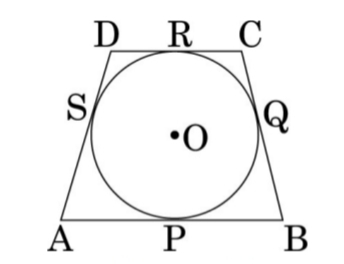
\includegraphics[width=\columnwidth]{./quadrilateralABCD.jpg}
        \caption{Quadrilateral ABCD}
        \label{fig:quadrilateralABCD}
    \end{figure}

    \item Solve for $x$:
    \begin{align}
        \sqrt{6x + 7} - (2x - 7) = 0
    \end{align}

    \item In \figref{fig:coneontopofcylinder}, a tent is in the shape of a cylinder surmounted by a conical top of the same diameter. If the height and diameter of the cylindrical part are $2.1 m$ and $3 m$ respectively, and the slant height of the conical part is $2.8 m$, find the cost of the canvas needed to make the tent if the canvas is available at the rate of $\rupee 500/ m^2$. (Use $\pi = \frac{22}{7}$)
    \begin{figure}[H]
	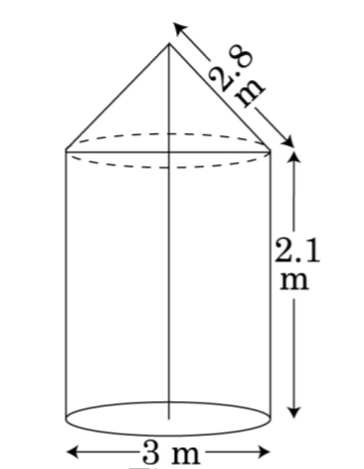
\includegraphics[width=\columnwidth]{./coneontopofcylinder.jpg}
        \caption{Cone on top of a cylinder}
        \label{fig:coneontopofcylinder}
    \end{figure}

    \item A sphere of diameter $12 cm$ is dropped in a right circular cylindrical vessel, partly filled with water. If the sphere is completely submerged in water, the water level in the cylindrical vessel rises by $3\frac{5}{9} cm$. Find the diameter of the cylindrical vessel.

    \item There are $100$ cards in a bag on which numbers from $1$ to $100$ are written. A card is taken out from the bag at random. Find the probability that the number on the selected card
    \begin{enumerate}
        \item is divisible by $9$ and is a perfect square.
        \item is a prime number greater than $80$.
    \end{enumerate}

    \item Three consecutive natural numbers are such that the square of the middle number exceeds the difference of the squares of the other two by $60$. Find the numbers.

    \item The sums of the first $n$ terms of three arithmetic progressions are $S_0, S_2$ and $S_3$ respectively. The first term of each A.P. is $1$ and their common differences are $1, 2$ and $3$ respectively. Prove that $S_1 + S_3 = 2S_2$.

    \item Due to heavy floods in a state, thousands were rendered homeless. Fifty schools collectively offered to provide place and canvas for $1500$ tents to be fixed by the government and decided to share the whole expenditure equally. The lower part of each tent is cylindrical with a base radius of $2.8 m$ and height $3.5 m$, with a conical upper part of the same base radius but of height $2.1 m$. If the canvas used to make the tents costs $\rupee 120/ m^2$, find the amount shared by each school to set up the tents. What value is generated by the above problem? (Use $\pi = \frac{22}{7} $)

    \item In \figref{fig:triangleABC}, the vertices of $\triangle ABC$ are $A(4, 6), B(1, 5)$ and $C(7, 2)$. A line segment $DE$ is drawn to intersect the sides $AB$ and $AC$ at $D$ and $E$ respectively such that $\frac{AD}{AB} = \frac{AE}{AC} = \frac{1}{3}$. Calculate the area of $\triangle ADE$ and compare it with the area of $\triangle ABC$.
    \begin{figure}[H]
        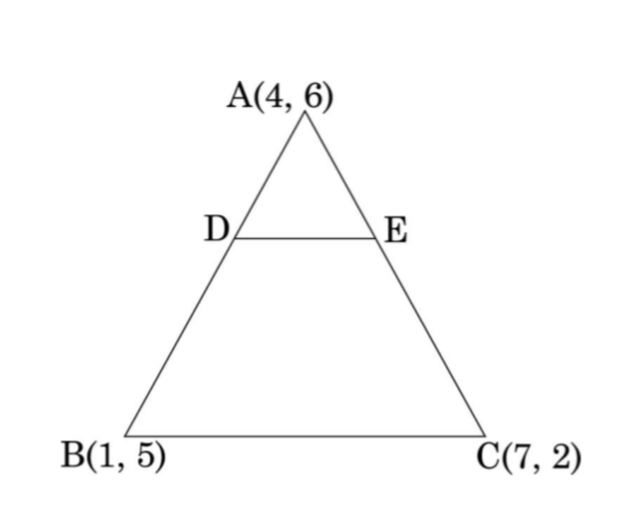
\includegraphics[width=\columnwidth]{./triangleABC.jpg}
        \caption{Triangle ABC}
        \label{fig:triangleABC}
    \end{figure}

    \item A motor boat whose speed is $24 km/hr$ in still water takes $1$ hour more to go $32 km$ upstream than to return downstream to the same spot. Find the speed of the stream.

    \item Two pipes running together can fill a tank in $11\frac{1}{9}$ minutes. If one pipe takes $5$ minutes more than the other to fill the tank separately, find the time in which each pipe would fill the tank separately.

    \item From a point on the ground, the angle of elevation of the top of a tower is observed to be $60^{\degree}$. From a point $40 m$ vertically above the first point of observation, the angle of elevation of the top of the tower is $30^{\degree}$. Find the height of the tower and its horizontal distance from the point of observation.

    \item Draw a triangle with sides $5 cm, 6 cm$ and $7 cm$. Then draw another triangle whose sides are $\frac{4}{5}$ of the corresponding sides of the first triangle.
\end{enumerate}
\end{document}
